%%
%% Copyright 2025 Oxford University Press
%%
%% This file is part of the 'oup-authoring-template Bundle'.
%% ---------------------------------------------
%%
%% It may be distributed under the conditions of the LaTeX Project Public
%% License, either version 1.3 of this license or (at your option) any
%% later version.  The latest version of this license is in
%%    https://www.latex-project.org/lppl.txt
%% and version 1.2 or later is part of all distributions of LaTeX
%% version 1999/12/01 or later.
%%
%% The list of all files belonging to the 'oup-authoring-template Bundle' is
%% given in the file `manifest.txt'.
%%
%% Template article for Oxford University Press's document class `oup-authoring-template'
%% with bibliographic references
%%

%%%CONTEMPORARY%%%
\documentclass[webpdf,contemporary,large]{oup-authoring-template}%
% \documentclass[unnumsec,webpdf,contemporary,large,numbered]{oup-authoring-template}% uncomment this line to get the numbered reference output
%\documentclass[unnumsec,webpdf,contemporary,medium]{oup-authoring-template}
%\documentclass[unnumsec,webpdf,contemporary,mediumone]{oup-authoring-template}
%\documentclass[unnumsec,webpdf,contemporary,small]{oup-authoring-template}

%%%MODERN%%%
%\documentclass[unnumsec,webpdf,modern,large]{oup-authoring-template}
%\documentclass[unnumsec,webpdf,modern,large,numbered]{oup-authoring-template}%   uncomment this line to get the numbered reference output
%\documentclass[unnumsec,webpdf,modern,medium]{oup-authoring-template}
%\documentclass[unnumsec,webpdf,modern,mediumone]{oup-authoring-template}
%\documentclass[unnumsec,webpdf,modern,small]{oup-authoring-template}

%%%TRADITIONAL%%%
%\documentclass[unnumsec,webpdf,traditional,large]{oup-authoring-template}
%\documentclass[unnumsec,webpdf,traditional,large,numbered]{oup-authoring-template}%   uncomment this line to get the numbered reference output
%\documentclass[unnumsec,webpdf,traditional,medium]{oup-authoring-template}
%\documentclass[unnumsec,webpdf,traditional,mediumone]{oup-authoring-template}
%\documentclass[namedate,webpdf,traditional,small]{oup-authoring-template}

%\onecolumn % for one column layouts

%\usepackage{showframe}
\newif\ifdraftnotes
\draftnotesfalse
\ifdraftnotes
  \usepackage{todonotes}
\else
  \usepackage[disable]{todonotes}
\fi
\newcommand{\revdone}[1]{\todo[inline,color=green!20,size=\footnotesize]{\textbf{REVIEW (applied):} #1}}
\newcommand{\revtodo}[1]{\todo[inline,color=orange!25,size=\footnotesize]{\textbf{REVIEW (action needed):} #1}}
\graphicspath{{fig/}}
\newif\ifshowfigures
\showfigurestrue

% line numbers
%\usepackage[mathlines, switch]{lineno}
%\usepackage[right]{lineno}
\usepackage{booktabs}
\usepackage{xurl}
\usepackage{xr}
\externaldocument[supp-]{supplementary}
\emergencystretch=1em
\usepackage{tikz}
\theoremstyle{thmstyleone}%
\newtheorem{theorem}{Theorem}%  meant for continuous numbers
%%\newtheorem{theorem}{Theorem}[section]% meant for sectionwise numbers
%% optional argument [theorem] produces theorem numbering sequence instead of independent numbers for Proposition
\newtheorem{proposition}[theorem]{Proposition}%
%%\newtheorem{proposition}{Proposition}% to get separate numbers for theorem and proposition etc.
\theoremstyle{thmstyletwo}%
\newtheorem{example}{Example}%
\newtheorem{remark}{Remark}%
\theoremstyle{thmstylethree}%
\newtheorem{definition}{Definition}

\usetikzlibrary{arrows.meta, positioning, shapes.geometric}

% Colors for overview figure
\definecolor{myblue}{HTML}{35beff}
\definecolor{mygreen}{HTML}{7edb73}
\definecolor{myred}{HTML}{ffa2ac}
\definecolor{mygene}{HTML}{FFB000}
\definecolor{mygo}{HTML}{FF7043}
\definecolor{myuberon}{HTML}{FFE082}
\definecolor{referencegray}{gray}{0.5}

% Inline circle commands (bullet-character style)
\newcommand{\bluecircle}{{\color{myblue}\raisebox{-0.3ex}{\scalebox{2}{$\bullet$}}}}
\newcommand{\greencircle}{{\color{mygreen}\raisebox{-0.3ex}{\scalebox{2}{$\bullet$}}}}
\newcommand{\redcircle}{{\color{myred}\raisebox{-0.3ex}{\scalebox{2}{$\bullet$}}}}
\newcommand{\genecircle}{{\color{mygene}\raisebox{-0.3ex}{\scalebox{2}{$\bullet$}}}}
\newcommand{\gocircle}{{\color{mygo}\raisebox{-0.3ex}{\scalebox{2}{$\bullet$}}}}
\newcommand{\uberoncircle}{{\color{myuberon}\raisebox{-0.3ex}{\scalebox{2}{$\bullet$}}}}

% Inline arrow commands for caption
\newcommand{\arrowsolid}{\tikz[baseline=-0.5ex]{\draw[->, thick, black!65] (0,0) -- (0.55,0);}}
\newcommand{\arrowmate}{\tikz[baseline=-0.5ex]{\draw[->, thick, purple!70!black] (0,0) -- (0.55,0);}}
\newcommand{\arrowdot}{\tikz[baseline=-0.5ex]{\draw[->, thick, black!35, dotted] (0,0) -- (0.55,0);}}
\newcommand{\arrowproje}{\tikz[baseline=-0.5ex]{\draw[->, thick, orange!80!black] (0,0) -- (0.55,0);}}
\newcommand{\arrowpred}{\tikz[baseline=-0.5ex]{\draw[->, thick, purple!70!black, dashed] (0,0) -- (0.55,0);}}

\newcommand{\method}{LinkGDA}

\newcommand{\projection}{OWL2Vec$^*$}
\newcommand{\projectionextended}{GDAProjector}
\renewcommand{\cite}{\citep}
\newcommand{\std}[1]{{\scriptsize $\pm$#1}}
\newcommand{\f}[1]{\textbf{#1}}
\newcommand{\s}[1]{\underline{#1}}

%\usepackage{draftwatermark}
%\SetWatermarkText{Draft}
%%Uncomment  \usepackage{draftwatermark} and \SetWatermarkText{Draft} to watermark your PDF as a draft
\begin{document}

\journaltitle{Bioinformatics}
\DOI{DOI added during production}
\copyrightyear{YEAR}
\pubyear{YEAR}
\vol{XX}
\issue{x}
\access{Published: Date added during production}
\appnotes{Paper}

\firstpage{1}

%\subtitle{Subject Section}

\title[PhenoQuery for gene--disease prediction]{PhenoQuery: phenotype-query learning and evaluation biases in gene--disease association prediction}

\author[1,3,4]{Fernando Zhapa-Camacho\ORCID{0000-0002-0710-2259}}
\author[2,3,4]{Naeema Muhammed\ORCID{0009-0007-1828-141X}}
\author[1,2,3,4]{Robert Hoehndorf\ORCID{0000-0001-8149-5890}}

\address[1]{\orgdiv{Computer, Electrical and Mathematical Sciences \&
    Engineering Division}, \orgname{King Abdullah University of Science and
    Technology}, \orgaddress{\street{4700 KAUST}, \postcode{23955},
    \state{Thuwal}, \country{Saudi Arabia}}}

\address[2]{\orgdiv{Biological and Environmental Science \&
     Engineering Division}, \orgname{King Abdullah University of
     Science and Technology}, \orgaddress{\street{4700 KAUST},
     \postcode{23955}, \state{Thuwal}, \country{Saudi Arabia}}}


\address[3]{\orgdiv{KAUST Center of Excellence for Smart Health
    (KCSH)}, \orgname{King Abdullah University of Science and
    Technology}, \orgaddress{\street{4700 King Abdullah University of
      Science and Technology}, \state{Thuwal}, \country{Saudi
      Arabia}}}

\address[4]{\orgdiv{KAUST Center of Excellence for Generative AI},
  \orgname{King Abdullah University of Science and Technology},
  \orgaddress{\street{4700 King Abdullah University of Science and
      Technology}, \state{Thuwal}, \country{Saudi Arabia}}}


\corresp[$\ast$]{Corresponding author.\href{mailto:robert.hoehndorf@kaust.edu.sa}{robert.hoehndorf@kaust.edu.sa}}

\received{Date}{0}{Year}
\revised{Date}{0}{Year}
\accepted{Date}{0}{Year}

%\editor{Associate Editor: Name}

\abstract{%
  \textbf{Motivation:} Predicting gene--disease associations for an unseen
  disease requires combining its phenotype profile with biological evidence
  about candidate genes. Relational graph foundation models can transfer this
  reasoning across graphs, but their use for gene ranking depends on how
  phenotype evidence is represented, combined, and evaluated.\\
  \textbf{Results:} We introduce PhenoQuery, which adapts ULTRA's relational
  graph network and UltraQuery's conjunctive query formulation to gene--disease
  prediction. PhenoQuery combines phenotype-to-gene projections on a graph
  augmented with typed Entity--Quality relations extracted from phenotype
  definitions. Across ten disease-disjoint folds and 13{,}625 candidate genes,
  typed Entity--Quality augmentation increases calibrated top-ten recovery
  from 11.93\% to 13.33\% relative to conjunction on the common ontology
  backbone (difference 1.40 percentage points; 99.5\% paired bootstrap interval
  0.35--2.41). In the same ULTRA-initialized campaign, removing intermediate
  training disease nodes increases top-ten recovery from 9.92\% to 11.43\%.
  We further analyze how candidate training status, phenotype overlap,
  calibration, and repeated profiles affect learned models and phenotype-based
  baselines. Of the test associations involving previously seen genes, 69.4\%
  share phenotypes with a training disease of the same gene. Per-gene
  calibration and status standardization improve unseen-gene recovery in
  selected models, while cohort restriction and profile weighting change
  the relative performance of the methods. These analyses identify the
  evaluation conditions under which phenotype-query learning improves
  gene ranking and quantify the effects of distinct scoring and evaluation
  adjustments.\\
  \textbf{Availability:} Source code, command-line workflows, and the
  reproducibility suite are available at
  \url{https://github.com/bio-ontology-research-group/link-gda}.\\
  \textbf{Contact:} \href{mailto:robert.hoehndorf@kaust.edu.sa}{robert.hoehndorf@kaust.edu.sa}\\
  \textbf{Supplementary information:} Supplementary methods and results
  accompany this manuscript.}

\keywords{gene--disease association, phenotype ontologies, inductive link
  prediction, knowledge graph embedding, benchmark debiasing, graph foundation models}

% \keywords[Abbreviations]{abbreviation1, abbreviation2, abbreviation3, abbreviation4}

% \otherabstract[Additional Abstract]{}

% \otherabstract[Graphical Abstract]{\colorbox{black!20}{\hbox to 0.97\textwidth{\vbox to 50pt{}}}}

% \boxedtext{Key Messages}{
% \begin{itemize}
% \item Key boxed text here.
% \item Key boxed text here.
% \item Key boxed text here.
% \end{itemize}}

\maketitle


%\begin{epigraph}
%Epigraph text. Ximporem qui reperov idempedit modio. Bisto imagnatem quae aceptis
%nobitae quid eum rae adignis quias-sit vellacc uptatur sunt quis rentis eaquasit alia deliquam
%rec-to consed unt. Empor sum ratur ressimusdae. Nam fugiae.
%\source{Epigraph source}
%\end{epigraph}

\section{Introduction}

Phenotype-based methods prioritize candidate genes for a disease by comparing
gene and disease phenotype profiles
\cite{kohler2009clinical,hoehndorf2011phenomenet,yuan2022evaluation}.
The Human Phenotype Ontology (HPO) \cite{gargano2024human}, Mammalian Phenotype
Ontology (MP) \cite{smith2009mammalian} and cross-species ontology UPheno
\cite{matentzoglu2024unified} allow human disease descriptions to be compared
with phenotypes of mouse orthologs. Mouse Genome Informatics (MGI)
\cite{baldarelli2024mouse} supplies these gene annotations, but missing profiles
prevent phenotype comparisons for some candidates. Gene Ontology (GO) function
annotations \cite{ashburner2000go,gocon2025} and tissue expression data such as
GTEx \cite{gtex2020} may help rank genes without phenotype profiles and improve
predictions for genes with phenotype profiles.

Clinical ontology- and network-based rankers such as Phrank
\cite{jagadeesh2019phrank} score phenotype overlap through conditional
information content. PhenoRank \cite{cornish2018phenorank} combines human
disease and mouse phenotype evidence with random walk with restart over
protein--protein interaction (PPI) networks. Graph representation learning methods extend this
paradigm to multi-modal knowledge graphs: DL2Vec \cite{chen2021predicting}
combines phenotype, function and expression knowledge in graph embeddings for
gene--disease prediction, and EmbedPVP \cite{althagafi2024prioritizing} combines
ontology embeddings with pathogenicity scores for variant prioritization. DL2Vec
learns disease representations during training, while EmbedPVP's inductive
variant fine-tunes embeddings for each new disease. INDIGENA \cite{indigena}
accepts a new disease profile without retraining by comparing learned phenotype
embeddings, but its scoring rule still requires gene phenotype profiles.
SHEPHERD \cite{alsentzer2025shepherd} learns from simulated patients over a
biomedical graph, and EvORanker \cite{canavati2024evoranker} uses phylogenetic
profiles to prioritize poorly annotated genes. Inductive relational graph
foundation models offer another approach: ULTRA \cite{ultra} transfers a
pretrained relational graph neural network to graphs with new entities and
relations, and UltraQuery \cite{galkin2024ultraquery} extends ULTRA to multi-hop
logical queries by combining link-prediction projections with fuzzy logical
intersection operators.

The interpretation of a ranking benchmark depends on how its queries and
reference annotations were constructed. Phrank uses conditional phenotype
information to account for shared ancestry and evaluates real patient profiles;
its authors also identify optimistic performance when simulated queries are
drawn from the same knowledgebase used for ranking \cite{jagadeesh2019phrank}.
PhenoRank addresses unequal study coverage by comparing each gene's observed
rank with ranks from simulated phenotype queries \cite{cornish2018phenorank}.
These methods establish important precedents for bias-aware evaluation. A
learned graph model introduces further choices about training disease nodes,
materialized gene--phenotype links, and the candidate universe.

We study these choices in disease-inductive prediction, where training and test
diseases are disjoint. A candidate gene can still have training disease
associations, and a new disease can share phenotypes with those training
diseases. We distinguish this available transfer evidence from prediction for
previously unseen genes or zero-overlap profiles. Repeated phenotype profiles
and diseases with multiple causal genes also affect how test associations
contribute to summary statistics.

We introduce PhenoQuery to combine phenotype evidence through conjunctive
queries over a relational graph network (Figure~\ref{fig:phenoquery}). Typed Entity--Quality relations connect
phenotype definitions to their biological entities and qualities, while
training disease nodes are excluded from the phenotype-query graph. Controlled
comparisons within a common initialization and adaptation protocol assess the
contributions of the graph representation and query readout. We then compare
learned graph models, Phrank, and PhenoRank under explicit candidate-status and
phenotype-overlap strata. Separate analyses measure the effects of per-gene
calibration, status standardization, duplicate reference profiles, co-causal
filtering, and evaluation weighting. This connects the proposed prediction
method to the biological evidence and evaluation conditions that support its
performance.

\ifshowfigures
% Editable vector source; requires tikz with arrows.meta and positioning.
\begin{figure*}[t]
\centering
\begin{tikzpicture}[
  font=\sffamily\small,
  box/.style={draw=black!45,rounded corners=2pt,align=center,inner sep=7pt},
  flow/.style={-{Latex[length=2mm]},thick,draw=black!65},
  note/.style={align=center,font=\sffamily\footnotesize},
  heading/.style={anchor=west,font=\sffamily\bfseries\small}
]
\node[heading] at (0,0) {(a) Build the phenotype-query graph};
\node[box,fill=blue!5,text width=4.9cm] (graph) at (2.6,-1.25)
  {Candidate genes + phenotype hierarchy\\[2pt]
   Gene--phenotype and gene--function edges\\
   Typed links from phenotype definitions};
\node[note,text width=4.9cm] at (2.6,-2.55)
  {Training: gene--phenotype links\\
   Query: disease phenotype set};
\node[box,fill=blue!5,text width=4.9cm] (encoder) at (2.6,-3.8)
  {Pretrained relational graph network\\[2pt]
   Evaluate initial and adapted models;\\select on validation diseases};
\draw[flow] (graph.west) -- ++(-.45,0) |- (encoder.west);

\node[heading] at (6.1,0) {(b) Rank genes for a disease phenotype set};
\node[box,text width=4.0cm] (query) at (8.5,-1.0)
  {Unseen disease\\$P_d=\{p_1,\ldots,p_m\}$};
\node[box,fill=blue!5,text width=4.0cm] (atomic) at (8.5,-2.65)
  {Project each phenotype to all genes\\$s(g,p_1),\ldots,s(g,p_m)$};
\node[box,fill=green!6,text width=4.0cm] (conjunction) at (8.5,-4.35)
  {Combine evidence by conjunction\\[2pt]
   $q(g,d)=\frac{1}{m}\sum_{p\in P_d}\log\sigma(s(g,p))$};
\draw[flow] (query) -- (atomic);
\draw[flow] (encoder.east) -- ++(.5,0) |- (atomic.west);
\draw[flow] (atomic) -- (conjunction);

\node[box,fill=green!6,text width=3.0cm] (calibration) at (13.1,-2.65)
  {Compare with the gene's\\reference-disease scores\\[2pt]
   $z(g,d)=\dfrac{q(g,d)-\mu_g}{\sigma_g+\epsilon}$};
\node[box,text width=3.0cm] (ranking) at (13.1,-4.35)
  {Rank all candidate genes\\[2pt]
   Retain raw and calibrated results};
\draw[flow] (conjunction.east) -- ++(.45,0) |- (calibration.west);
\draw[flow] (calibration) -- (ranking);

\node[heading] at (0,-5.75) {(c) Audit the scoring rule and evaluation population};
\node[box,text width=4.25cm] at (2.4,-6.75)
  {Training-association status\\[2pt]
   Seen/unseen strata and within-status ranks};
\node[box,text width=4.25cm] at (7.55,-6.75)
  {Training-phenotype overlap\\[2pt]
   Shared phenotypes and zero-overlap cohort};
\node[box,text width=4.25cm] at (12.7,-6.75)
  {Repeated profiles and positives\\[2pt]
   Reference deduplication, co-causal filtering and profile weighting};
\end{tikzpicture}
\caption{PhenoQuery and its evaluation.
(a) The typed PhenoQuery graph combines gene annotations, ontology hierarchy
and typed Entity--Quality links extracted from phenotype definitions. Its
standard construction omits training disease nodes and expression edges;
a separate disease-bridge arm tests the effect of retaining training diseases.
(b) Each query phenotype supplies an atomic gene-link score. Length-normalized
log-sigmoid conjunction combines these scores, and per-gene reference
calibration adjusts their baseline level and scale. The query disease is
excluded from its calibration reference panel.
(c) Training status, phenotype overlap and repeated profiles define distinct
score adjustments or evaluation sensitivities. Their effects are reported
separately, with each analysis retaining its defined scoring rule and population.}
\label{fig:phenoquery}
\end{figure*}

\fi

\section{Methodology}

\subsection{Data sources and benchmark construction}
\label{sec:datasets}

We combine mouse gene--phenotype associations and human orthology from
MGI \cite{baldarelli2024mouse}; disease phenotypes and human gene--disease
associations from HPO release \texttt{v2026-01-08}
\cite{gargano2024human}; gene functions from GO
\cite{ashburner2000go,gocon2025}; and anatomical expression from GTEx
\cite{gtex2020}. UPheno version~2, release \texttt{2025-10-12}
\cite{matentzoglu2024unified}, aligns MP and HPO phenotype terms, while
GO and UBERON \cite{mungall2012uberon} provide the function and anatomy
classes. Suppl. Table~\ref{supp-tab:datasets} gives the prepared input counts.

For the main benchmark, we retained gene--disease pairs whose gene
had at least one MGI-derived phenotype annotation and whose disease
had at least one HPO annotation, with both profiles represented in
UPheno. This yielded 6{,}571 associations involving 6{,}059 diseases.
We rank 13{,}625 genes with at least one phenotype represented in UPheno;
candidate eligibility is independent of disease-association labels.
Requiring gene phenotype annotations supports comparison with the
phenotype-based baselines.

We also test whether gene function and expression sites support ranking when
gene phenotype profiles are unavailable. In the controlled setting, we
deliberately withhold available gene phenotype annotations from the main
benchmark, using the same associations and candidate genes as specified in
Section~\ref{sec:graph}. In the excluded-gene benchmark, the genes have no
phenotype annotations in the MGI source data.

Withholding annotations from characterized genes may not reflect performance
on genes that lack those annotations. For the second setting, we
constructed the excluded-gene benchmark from pairs excluded
because the gene lacked an MGI-derived phenotype profile; the main benchmark
supplies its training associations. We retained genes
with GO functions and diseases with HPO phenotypes, then excluded diseases in
the main benchmark and those with phenotype-set Jaccard similarity of at least
0.5 to a main-benchmark disease. The resulting benchmark contains 425
associations involving 364 genes and 417 diseases. The primary candidate pool
contains all 5{,}696 GO-annotated genes without MGI phenotype annotations.
A secondary analysis ranks all 18{,}904 GO-annotated genes. Both pools use
annotation eligibility independently of the test associations.
The Supplementary Material gives source files, access dates,
identifier mapping, annotation filters and excluded-gene benchmark counts
after each filtering step.




\subsection{Knowledge graph construction}
\label{sec:graph}

We represent the ontology classes, genes and
training diseases as entities in a directed, labelled graph
(Suppl. Fig.~S1a). We add gene--disease associations as
\texttt{associated\_with} edges and disease--phenotype annotations as
\texttt{has\_symptom} edges. Gene annotations supply
\texttt{has\_phenotype} edges to MP classes, \texttt{has\_function}
edges to GO classes, and \texttt{expressed\_in} edges to UBERON
classes, according to the modalities included in each variant.
Test diseases and their association and phenotype edges are excluded
from the training graph.



We project UPheno into graph edges with
\projection{} \cite{owl2vecstar}, and additionally project GO when
function annotations are included and UBERON when expression
annotations are included. Each ontology is projected in a fresh process using
mOWL v1.0.3, with bidirectional taxonomy edges and without literals. We
deduplicate projected edges and the assembled training triples.

To test whether explicit cross-ontology Entity--Quality (EQ) links improve
multi-hop message passing between phenotype classes and gene function or
anatomy annotations, we also construct an EQ-augmented graph. Because the
default \projection{} projection of UPheno retains taxonomy edges together with
only two existential object properties (\texttt{UPHENO:0000001} and
\texttt{RO:0002573}), we parse the pinned UPheno OWL ontology to extract all
named-class subclass restrictions $A \sqsubseteq \exists r.B$ and logical
equivalence intersections $A \equiv G \sqcap \sqcap_i \exists r_i.B_i$ linking
HP, MP or UPheno classes to GO, UBERON or PATO classes. We evaluate three
incremental projection modes: (i) \texttt{entity}, which collapses existential
links into a single cross-ontology relation; (ii) \texttt{typed}, which
preserves the distinct relation IRI $r$ of each existential restriction; and
(iii) \texttt{structure}, which introduces reified blank nodes for nested
role-chain filler structures. In our matched ULTRA and UltraQuery comparisons,
augmenting the base graph (215{,}936 nodes, 14 forward relations, 1{,}916{,}526
forward edges in fold 0) with the union of \texttt{entity} and \texttt{typed}
EQ projections adds 1{,}923 PATO quality classes, 26 forward relation types
(80 total directed relations including inverses), and 148{,}798 forward edges
(2{,}065{,}324 total forward edges).

For each training association between a gene $g$ and a disease $d$, we
materialize each disease phenotype $p$ as a direct
$(g,\texttt{causes\_phenotype},p)$ triple. These triples provide the
supervised gene--phenotype relation used to score candidate genes for
unseen diseases and use only training associations and phenotypes. Because
retaining training disease nodes and their \texttt{associated\_with} and
\texttt{has\_symptom} edges creates two-hop hubs connecting training genes to
entire disease syndromes, we also construct a phenotype-only graph variant
(\texttt{plain}, \texttt{entity}, \texttt{typed}, and \texttt{structure}) that
removes all disease nodes and incident \texttt{associated\_with} and
\texttt{has\_symptom} edges while retaining the materialized
\texttt{causes\_phenotype} triples, gene annotations, and ontology projections.

The suffixes p, f and s denote inclusion of
mouse-derived gene phenotypes, GO functions and anatomical expression
sites, respectively. We evaluate \method{}-p, -f, -s, -pf, -ps, -fs
and -pfs. We refer to the full three-modality model, \method{}-pfs, as
\method{}. In the controlled phenotype-withheld variants, genes represented by
another included modality have their phenotype edges withheld; when no other
included annotation is available, we retain one eligible phenotype edge so the
gene remains represented. These variants retain training gene--disease
associations and their materialized \texttt{causes\_phenotype} links, so
withholding a gene's phenotype profile does not remove training-derived
phenotype supervision. Genes in the excluded-gene benchmark lack
MGI-derived phenotype annotations. The Supplementary Methods specify the fallback rule and its coverage;
retained graph manifests identify the exact training triples.

\subsection{Relational phenotype-query models and adaptation}

ULTRA~\cite{ultra} and UltraQuery~\cite{galkin2024ultraquery} share a
168{,}705-parameter relational graph neural network architecture comprising a
6-layer, 64-dimensional Bellman-Ford relation-interaction network over the four
fundamental relation-graph interactions (head-to-head, tail-to-tail,
head-to-tail and tail-to-head) followed by a 6-layer, 64-dimensional entity
Bellman-Ford network with DistMult message functions, sum aggregation, layer
normalization and a two-layer MLP link scorer. Both models score each query
phenotype $p \in P_d$ in the reverse direction
$(p, \texttt{causes\_phenotype}^{-1}, g)$ so that a single Bellman-Ford pass
seeded at $p$ scores all 13{,}625 candidate genes simultaneously. The
general-domain checkpoint \texttt{ultra\_4g} is pretrained on single-hop link
prediction across four knowledge graphs, whereas \texttt{ultraquery} is
additionally fine-tuned on multi-hop logical queries using product-t-norm
intersections. In our primary zero-shot comparison (Table~\ref{tab:rq1}),
\texttt{ultra\_4g} is evaluated without fine-tuning using fixed BMA
(Equation~\ref{eq:bma}) and per-gene calibration (Equation~\ref{eq:calibration}).

To evaluate pooling versus conjunctive intersection, EQ ontology projections,
and domain adaptation under identical conditions, we run a matched three-stage
curriculum for both \texttt{ultra\_4g} (\texttt{general}) and
\texttt{ultraquery} (\texttt{query}) across all ten folds:
\begin{enumerate}
\item In Stage~1 (frozen readout selection), we score all validation disease
  phenotypes with the frozen checkpoint and select the pooling weight
  $w \in \{0.0, 0.1, \dots, 1.0\}$ (Equation~\ref{eq:pool}) or intersection
  input temperature $T_{\mathrm{in}} \in \{2^{-4}, \dots, 2^{6}\}$
  (Equation~\ref{eq:and}), together with the scoring mode (raw or disease-level
  calibrated), by lexicographic validation performance on
  $(\mathrm{H@10}, \mathrm{H@1}, \mathrm{MRR}, -\mathrm{MR})$.
\item In Stage~2 (candidate-gene link fine-tuning), we fine-tune the backbone
  for up to 1{,}000 steps (AdamW, learning rate $5\times 10^{-5}$, weight decay
  $10^{-4}$, 100-step linear warmup, cosine decay, gradient norm clipping 1.0,
  batch size 8 phenotypes) using a balanced binary cross-entropy loss over all
  known training positive genes $G^{+}(p)$ of a sampled phenotype $p$ and 64
  uniformly sampled negative candidate genes from
  $\mathcal{G}_{\mathrm{cand}} \setminus G^{+}(p)$. Every batch masks all
  direct $(g, \texttt{causes\_phenotype}, p)$ and inverse edges for its queried
  phenotypes so the model must predict through multi-hop ontology and
  annotation paths. Checkpoints are evaluated every 200 steps on validation
  diseases under both \texttt{Pool} and \texttt{AND} readouts.
\item In Stage~3 (full-profile ranking fine-tuning), we initialize from the
  best Stage~1/2 checkpoint for each readout and train for up to 500 steps
  (AdamW, learning rate $2\times 10^{-5}$, 50-step warmup, evaluated every 100
  steps) directly on training disease profiles $P_d$. For each sampled training
  disease $d$, we mask all direct $\texttt{causes\_phenotype}$ and inverse
  edges for every $p \in P_d$ across all genes (label-independent masking) as
  well as all $\texttt{associated\_with}$ and $\texttt{has\_symptom}$ edges
  incident to $d$. We optimize a multi-positive sampled softmax loss with
  output temperature $T_{\mathrm{out}} \in \{0.01, 0.1, 1.0, 10.0\}$ over all
  positive genes $G^{+}(d)$ and 64 negative candidate genes (32 uniform plus 32
  hard negatives mined from 256 candidate proposals) using exact two-pass
  chain-rule gradient replay across $p \in P_d$.
\end{enumerate}
For the phenotype-query campaign, all nine graph/readout arms start from
\texttt{ultra\_4g}. We use UltraQuery's QueryNBFNet projection architecture with
a mean log-sigmoid conjunction evaluated directly in log space. Each arm uses
500 sampled-softmax profile updates, with validation at initialization and every
100 updates. Checkpoint selection retains initialization as a fallback and
requires eligible updates to preserve both validation Hits@1 and Hits@10.
The selected checkpoints, including fallbacks, are reported with their update
counts in the reproduction artifacts.

\subsection{Embedding-model comparators and training}
\label{sec:lp}

We train TransD \cite{ji2015knowledge} on each graph to learn entity and
relation embeddings and score the supervised relations. Its entity- and
relation-specific projections support the graph's many-to-many relations.

We train one model per fold with the
Adam optimizer \cite{diederik2014adam} and stop when validation mean
rank stops improving. In each cross-validation split, we reserve one fold
for testing and select 10\% of the diseases from the remaining nine folds
for validation. Validation diseases retain their phenotype annotations in the
graph, but their gene associations are withheld. These withheld
associations contribute no \texttt{associated\_with} edge and no materialized
\texttt{causes\_phenotype} edge. Validation ranks candidate genes
following the same procedure as the test evaluation. Test diseases are
absent from the graph altogether.


We freeze each TransD variant's embedding dimension, batch size and learning
rate before the evaluation runs, using the study's historical calibrated-setting
configuration. Within that configuration, we retain checkpoints selected by
raw and calibrated validation mean rank and evaluate both scoring rules on
each checkpoint. This separates the effect of checkpoint selection from the
effect of score transformation. We use training seed 0 for the ten main folds
and seeds 0--9 for the excluded cohort, with validation split seed 0 throughout.
For the excluded cohort, checkpoint selection uses validation associations
whose genes have no training association, ranked against the full GO pool.
Suppl. Table~\ref{supp-tab:configurations} lists the fixed configurations and their historical selection
protocol, including a sensitivity excluding reconstructed tuning diseases.

We also evaluate ConvKB-D \cite{nguyen-etal-2018-novel,indigena}, initialized
from the calibrated-selected TransD checkpoint for the matching fold and seed.
Its raw and calibrated configurations remain separately fixed. To test how the
negative-sampling distribution during TransD training affects top-ranked
retrieval and training-status offsets, we additionally evaluate two
candidate-pool training variants of \method{}-pfs: \texttt{T1}, which restricts
head-entity negative sampling on \texttt{causes\_phenotype} triples to the
13{,}625 candidate genes; and \texttt{P-pool}, which fine-tunes the
\texttt{causes\_phenotype} scoring head directly on training disease phenotype
profiles using uniform and hard-negative candidate genes. The scoring
functions, configurations and training budgets are specified in the
Supplementary Methods.

\subsection{Gene scoring and calibration}
\label{sec:scoring}

To score a candidate gene $g$ against a
test disease $d$ with phenotypes $P_d$, we define the link prediction
score for a single phenotype $p$ as:
\begin{equation}
  s(g, p) = f(g,\,\texttt{causes\_phenotype},\,p),
\end{equation}
where $f$ is the scoring function of the trained TransD or ConvKB-D model.
Higher values indicate a stronger predicted association.

We aggregate $s(g, p)$ over $P_d$ with a
Best-Match Average (BMA):
\begin{equation}
  \label{eq:bma}
  \text{score}(g, d) = \frac{1}{2}\!\left(
    \max_{p \in P_d} s(g, p)
    \;+\;
    \frac{1}{|P_d|}\sum_{p \in P_d} s(g, p)
  \right).
\end{equation}
This is BMA specialized to a single gene entity and the disease phenotype set.
\method{} scores the gene directly against the disease's phenotypes through
the learned \texttt{causes\_phenotype} relation. Semantic-similarity methods
and INDIGENA \cite{indigena} instead compare the gene's phenotype set with
the disease's phenotype set.

For relational graph foundation models, we also evaluate two parameterized
phenotype-set readouts that generalize fixed BMA. The first is a learned convex
pooling combination (\texttt{Pool}) of the maximum and mean phenotype scores:
\begin{equation}
  \label{eq:pool}
  \text{score}_{\mathrm{pool}}(g, d) = w \max_{p \in P_d} s(g, p)
    \;+\; (1 - w)\frac{1}{|P_d|}\sum_{p \in P_d} s(g, p),
\end{equation}
where $w \in \{0.0, 0.1, \dots, 1.0\}$ is selected on validation diseases. The
second is a conjunctive query intersection readout (\texttt{AND}) that treats
the disease profile $P_d$ as the logical conjunction of $|P_d|$ atomic link
queries $\exists g.\,\bigwedge_{p \in P_d}\texttt{causes\_phenotype}(g, p)$ and
combines per-phenotype link probabilities via a length-normalized log-space
product t-norm:
\begin{equation}
  \label{eq:and}
  \text{score}_{\mathrm{and}}(g, d) = \frac{1}{|P_d|}\sum_{p \in P_d}
    \log \sigma\!\left(\frac{s(g, p)}{T_{\mathrm{in}}}\right),
\end{equation}
where $\sigma(x) = (1 + e^{-x})^{-1}$ is the logistic sigmoid and
$T_{\mathrm{in}} \in \{2^{-4}, 2^{-3}, \dots, 2^{6}\}$ is an input temperature
selected on validation diseases to prevent probability saturation and numerical
underflow across variable-length phenotype profiles.

Genes can receive consistently high or low
scores across queries, partly related to whether they appear in training
associations. Per-gene calibration compares each query score with that gene's
usual score level and variation:
\begin{equation}
  \label{eq:calibration}
  z(g, d) = \frac{\text{score}(g, d) - \mu_g}{\sigma_g + \epsilon},
\end{equation}
where $\mu_g$ and $\sigma_g$ are the population mean and standard
deviation of gene $g$'s scores over distinct reference diseases, and
$\epsilon=10^{-12}$. Our batch evaluation uses the other diseases in the test
fold as the reference panel, with one vector per disease regardless of its
number of associated genes. The query disease is omitted completely. This
standardization produces a relative ranking score. We apply it identically to
learned and semantic-similarity methods.

For deployment on a single new disease, we also compute fixed statistics from
the distinct training diseases and apply them to each test query. Reference
identities and candidate order are retained with the statistics. This panel
contains training-derived phenotype links and therefore evaluates a different
reference distribution from the test-disease panel.

Because per-gene calibration standardizes each gene across reference diseases,
it removes static gene-level offsets while preserving within-query variance and
tail differences between training-associated (\emph{seen}) and unassociated
(\emph{unseen}) candidate genes. To remove query-specific location and scale
differences between the two status strata in the full 13{,}625-gene pool, we
define within-query status-stratum standardization (\texttt{Status-Z}):
\begin{equation}
  \label{eq:status_z}
  \tilde{z}(g, d) = \frac{z(g, d) - \mu_{d,\mathrm{status}(g)}}{\sigma_{d,\mathrm{status}(g)} + \epsilon},
\end{equation}
where $\mu_{d,\mathrm{status}(g)}$ and $\sigma_{d,\mathrm{status}(g)}$ are the
mean and standard deviation of $z(g', d)$ over all candidate genes $g'$ in the
same training-association stratum as $g$ ($\mathcal{G}_{\mathrm{seen}}$ or
$\mathcal{G}_{\mathrm{unseen}}$) for query disease $d$. This transformation
forces the seen and unseen candidate sub-pools to have zero mean and unit
variance on every query while preserving continuous score separation near the
top of each stratum. In addition, because distinct diseases can share an
identical phenotype set $P_d = P_{d'}$, we define deduplicated
leave-one-profile-out calibration (\texttt{Dedup-LOO}), which collapses
identical phenotype profiles in the reference panel to unit weight and excludes
all diseases sharing $P_d$ when computing $\mu_g$ and $\sigma_g$ for query $d$.

\subsection{Evaluation protocol and statistical analysis}
\label{sec:eval}

We adopt an inductive evaluation
protocol where test diseases are absent from the training graph. We
partition diseases into ten subsets of approximately equal size and
apply ten-fold cross-validation: in each fold, the diseases in nine
subsets and their gene associations are used for training and the
remaining subset is held out for testing. Because the split is by
disease, the number of gene--disease pairs per fold varies. Test
diseases do not appear as nodes in the training graph and their
gene--disease associations are never observed during training. For the original
embedding-model comparison, we train one model per fold at a fixed seed and
report each metric as a mean and standard deviation over the ten folds.
This spread measures variation across held-out disease sets. The
phenotype-query component contrasts pool associations across folds;
their bootstrap intervals and the equal-fold summaries are labelled separately.

The excluded-gene experiment uses one disease-disjoint split and ten training
seeds. Variation across seeds describes optimization variability on this fixed
cohort. The main ten-fold analysis describes variation across held-out diseases.

For every query, each method ranks the same annotation-defined candidate pool.
We use unfiltered ranks: other known positive genes for a disease remain
candidates. Tied scores receive their average rank. The primary endpoint of the
original embedding-model comparison is association-pair mean rank (MR).
The phenotype-query component analysis focuses on Hits at 10. We also report
mean reciprocal rank (MRR),
Hits at 1, 3, 10 and 100, candidate-percentile thresholds, disease-averaged
metrics, medians and rank cumulative distribution functions. We define the
rank-based AUC as $(N-\mathrm{MR})/(N-1)$ for $N$ candidates. Filtered ranks
are a sensitivity analysis.

The original embedding-model comparison tests calibrated \method{} against INDIGENA,
ConvKB-D and zero-shot ULTRA. We apply paired two-sided Wilcoxon signed-rank
tests to the ten fold MRs, with Holm adjustment across these three comparisons.
Overlapping training sets can correlate fold outcomes, which limits the
interpretation of these tests. The benchmark also informed method development,
so these comparisons describe performance on the reused benchmark.
For the excluded cohort, we compare the
function and function--expression variants with matched ULTRA variants. We
average each association's ranks over seeds, then bootstrap whole diseases
10{,}000 times with seed 20261013. Each of the two differences has a 97.5\%
percentile interval, giving Bonferroni family coverage of 95\%. Other
comparisons are descriptive sensitivity analyses.

To quantify candidate-composition effects, we include query-independent rules
that rank seen or unseen training genes first and rules based on annotation
counts. We additionally rerank each true gene among candidates sharing its
training-association status, using the scores calibrated in the original
reference panel. This removes rank gains attributable solely to an additive
score difference between the two status groups. Annotation-count strata retain
the full candidate pool.

\subsection{Baselines}
\label{sec:baselines}

All baselines use the same inductive splits, candidate pools, and
gene--disease pairs as \method{} within each benchmark.

We use the information-content measures Resnik
\cite{resnik1995using} and Lin \cite{linsemsim} combined with Best-Match
Average (BMA) aggregation
\cite{pesquita2009semantic}, and the group-wise measure SimGIC
\cite{pesquita2007evaluating}. These
operate directly on phenotype sets and are inherently inductive.

Exomiser-Phive \cite{robinson2014improved} scores a
candidate gene from the phenotypes of its mouse ortholog. Phive uses the
phenotype annotations distributed with Exomiser. The other
phenotype-only Exomiser prioritizers use known human disease--gene
associations, including the evaluated pairs, so they do not match this
inductive protocol.

INDIGENA \cite{indigena} scores using phenotype embeddings
and ranks a candidate gene by a best-match aggregation of
similarities between the gene's and the disease's phenotype
embeddings. We apply that rule to our graphs using its fixed historical calibrated-setting configuration.

Phrank \cite{jagadeesh2019phrank} and PhenoRank
\cite{cornish2018phenorank} provide ontology-similarity and network-propagation
comparators with fold-specific human annotations. Native HPO Phrank uses the
author implementation to sum marginal information content over the shared
ancestor closure of disease and gene phenotype sets. Its gene annotations and
information content use only inner-training disease--gene associations. We
evaluate both the direct-gene readout, which unites a gene's training phenotype
annotations, and the published disease-max readout, which takes the maximum
similarity over its training diseases. We report their raw scores separately.
We extract explicit named HPO subclass axioms from the retained ontology snapshot,
retain unknown query terms as singleton nodes, and assign unannotated genes
zero evidence. All 13{,}625 genes remain candidates, with average-rank ties.

Separate Phrank adaptations use UPheno ancestry with human-only, human-plus-MGI,
or MGI-only annotations. Direct scoring unites the permitted phenotype
annotations of each gene; disease-max scoring takes the maximum over its
training-disease profiles and, where applicable, its mouse phenotype profile.
We retain native information-content overlap and report annotation-normalized
scores as an additional sensitivity. The human-only UPheno arm and the native
HPO arm use different ontology hierarchies. Mouse-only scoring provides a
comparison whose gene annotations are independent of human training associations.

PhenoRank initializes gene scores from information-content-weighted phenotype
similarity, applies 20 random-walk-with-restart iterations with restart
probability 0.1, and compares each observed gene's ascending rank against ranks
from 1{,}000 simulated phenotype queries. The empirical probability is the
fraction of null ranks at least as large as the observed rank, with floor
$1/1000$. We retain the published decreasing-co-occurrence-tier sampler,
including replacement within partially sampled tiers. The historical-resource
adapter retains the archived mouse and PPI evidence while rebuilding human
annotations, information content and simulation co-occurrence within each fold.
Ontology-based mapping to its archived vocabulary and candidate-universe
extension are specified in the Supplementary Methods.

UPheno PhenoRank adaptations compare additive human-plus-mouse scoring
(\texttt{HM-Add+PPI}), averaging across the available human and mouse sources
(\texttt{HM-Bal+PPI}), mouse-only scoring with PPI propagation
(\texttt{Mouse+PPI}), and mouse-only scoring without propagation
(\texttt{Mouse-NoPPI}). These adaptations share null simulations among queries
of the same requested phenotype-set size. We report negative empirical
probabilities, an observed-rank tie-breaking sensitivity, and continuous
pre-simulation scores separately. The native historical-resource adapter
simulates independently for each query.

The knowledge-graph embedding sensitivities include graphs with training
disease entities and graphs with those entities and their incident edges
removed. Materialized gene--phenotype links and the remaining annotations are
retained. The existing U1, T1, profile-ranking, ConvKB-D and INDIGENA
configurations provide descriptive comparisons across training and selection
settings; their dimensions, budgets, negative-sampling filters and checkpoint
criteria differ and are specified with the corresponding results.

The separate fixed-checkpoint ULTRA sensitivity analysis removes either edges
incident to training disease nodes or expression edges from the entity graph.
It retains the node inventory, relation-interaction graph, and pretrained
weights. The direct-overlap score-aggregation control omits cached
phenotype--gene scores corresponding to training phenotype overlap and uses a
background mean when no query entries remain. Paired comparisons use 10{,}000
disease-cluster bootstrap replicates (seed 20261013), with the reported interval
level adjusted for the specified family of contrasts.

Query-independent annotation controls rank genes by the numbers of distinct
phenotype, function or expression annotations. The Supplementary Methods
specify these controls and the training-status comparisons.


\section{Results}

\subsection{Typed phenotype queries improve top-ten gene retrieval}
\label{sec:ultraquery_results}

PhenoQuery combines a relational graph network with phenotype conjunction
and typed entity--quality links. We compared its components within the
ULTRA-initialized campaign, using the same optimization and validation rules
for each arm (Table~\ref{tab:ultra_matched}). Removing training disease nodes
from the pooling arm increased association-pooled calibrated Hits@10 from
9.92\% to 11.43\%, a gain of 1.51 percentage points (99.5\% disease-bootstrap
interval 0.69--2.34). Mean rank improved from 2{,}232.8 to 2{,}153.7. This
contrast supports the disease-free graph for phenotype-query learning under
the evaluated training protocol.

Conjunction and typed ontology links contributed at different ranking
endpoints. Replacing pooling with mean log-sigmoid conjunction increased
Hits@1 from 2.02\% to 2.69\%; its Hits@10 difference was 0.50 percentage points
(99.5\% interval $-0.73$ to $1.72$). Adding typed entity--quality links to
conjunction increased Hits@10 from 11.93\% to 13.33\%, a gain of 1.40 points
(99.5\% interval 0.35--2.41), and improved mean rank from 1{,}875.7 to
1{,}805.2. The corresponding Hits@1 difference was 0.40 points (99.5\%
interval $-0.23$ to $1.01$). The clearest contribution of typed EQ information
in this campaign is improved top-ten recovery.

\begin{table*}[tb]
\centering\small
\caption{Historical matched ULTRA and UltraQuery comparison and ULTRA-initialized PhenoQuery component study (ten disease folds, 6,571 test associations, 13,625 candidates). MR is the equal-fold mean $\pm$ sample standard deviation; Median pools associations; MRR and Hits@k are equal-fold means. Seen and Unseen MR pool associations within each status ($n=3{,}085$ and $n=3{,}486$). Primary denotes validation-selected scoring in the matched campaign. Panel B initializes every arm from \texttt{ultra\_4g}; it does not compare initialization effects.}
\label{tab:ultra_matched}
\begin{tabular}{llrrrrrrr}
\toprule
Variant & Scoring & MR & Median & MRR & H@1 (\%) & H@10 (\%) & Seen MR & Unseen MR \\
\midrule
\multicolumn{9}{l}{\emph{Panel A: Matched graphs, readouts and adaptation stages}} \\
ULTRA, original, Pool, frozen & Cal.\ (Primary) & 2120.83\std{72.92} & 271 & 0.081 & 4.08 & 16.04 & 1555.92 & 2621.52 \\
ULTRA, original, Pool, adapted & Cal.\ (Primary) & 2129.99\std{78.34} & 271 & 0.080 & 3.95 & 15.72 & 1572.22 & 2624.29 \\
ULTRA, original, Pool, adapted & Raw & 3044.19\std{358.87} & 2234 & 0.051 & 2.66 & 9.82 & 618.02 & 5190.63 \\
ULTRA, original, AND, adapted & Cal.\ (Primary) & 2131.87\std{81.81} & 273 & 0.080 & 3.95 & 15.65 & 1574.28 & 2626.02 \\
ULTRA, EQ-aug., Pool, adapted & Cal.\ (Primary) & 1976.27\std{103.58} & 281 & 0.077 & 3.83 & 15.28 & 1407.10 & 2481.43 \\
ULTRA, EQ-aug., AND, adapted & Cal.\ (Primary) & 1976.14\std{103.70} & 282 & 0.077 & 3.79 & 15.22 & 1407.66 & 2480.71 \\
UltraQuery, original, Pool, frozen & Raw (Primary) & 3619.36\std{191.36} & 2493 & 0.068 & 4.40 & 11.49 & 1898.73 & 5149.12 \\
UltraQuery, original, Pool, frozen & Cal.\ & 3676.00\std{220.62} & 2019 & 0.057 & 3.02 & 10.71 & 2327.49 & 4873.04 \\
UltraQuery, original, Pool, adapted & Raw (Primary) & 2871.58\std{280.45} & 1398 & 0.076 & 4.91 & 13.00 & 943.26 & 4575.62 \\
UltraQuery, original, Pool, adapted & Cal.\ & 2864.60\std{476.21} & 784 & 0.061 & 3.31 & 11.46 & 1856.52 & 3756.31 \\
UltraQuery, original, AND, adapted & Raw (Primary) & 3272.95\std{466.30} & 2057 & 0.074 & 4.72 & 12.57 & 895.34 & 5368.32 \\
UltraQuery, EQ-aug., Pool, adapted & Raw (Primary) & 2920.27\std{223.91} & 1466 & 0.077 & 4.94 & 13.24 & 712.10 & 4874.67 \\
UltraQuery, EQ-aug., Pool, adapted & Cal.\ & 2659.07\std{261.80} & 741 & 0.060 & 3.17 & 11.58 & 1780.78 & 3444.18 \\
UltraQuery, EQ-aug., AND, frozen & Cal.\ (Primary) & 2282.93\std{135.06} & 520 & 0.076 & 4.49 & 13.52 & 1493.10 & 2985.28 \\
UltraQuery, EQ-aug., AND, adapted & Cal.\ (Primary) & 2299.30\std{163.53} & 505 & 0.076 & 4.60 & 13.59 & 1489.00 & 3020.40 \\
UltraQuery, EQ-aug., AND, adapted & Raw & 2919.47\std{424.89} & 1362 & 0.070 & 4.27 & 12.38 & 901.72 & 4707.16 \\
\midrule
\multicolumn{9}{l}{\emph{Panel B: ULTRA-initialized PhenoQuery component campaign}} \\
PhenoQuery, \texttt{bridge\_pool} & Cal.\ & 2233.50\std{99.41} & 354 & 0.046 & 1.76 & 9.92 & 1613.07 & 2781.28 \\
PhenoQuery, \texttt{bridge\_pool} & Raw & 2520.13\std{345.52} & 1137 & 0.061 & 3.16 & 12.06 & 533.97 & 4289.16 \\
PhenoQuery, \texttt{plain\_pool} & Cal.\ & 2152.85\std{134.17} & 281 & 0.053 & 2.03 & 11.43 & 1543.76 & 2693.42 \\
PhenoQuery, \texttt{plain\_and} & Cal.\ & 1874.68\std{137.30} & 306 & 0.060 & 2.69 & 11.93 & 1491.26 & 2215.83 \\
PhenoQuery, \texttt{entity\_and} & Cal.\ & 1872.08\std{119.64} & 282 & 0.062 & 2.85 & 12.47 & 1448.00 & 2248.68 \\
PhenoQuery, \texttt{typed\_and} & Cal.\ & 1803.10\std{143.57} & 252 & 0.066 & 3.10 & 13.34 & 1493.25 & 2081.32 \\
\bottomrule
\end{tabular}
\end{table*}


The separate matched ULTRA/UltraQuery experiment evaluates the general-domain
and logical-query-pretrained checkpoints under a shared adaptation curriculum
(Suppl.\ Tables~\ref{supp-tab:ultra_full} and~\ref{supp-tab:ultra_full_query}). Its selected readouts and scoring transformations vary
across configurations. PhenoQuery's nine-arm component experiment uses the
general-domain \texttt{ultra\_4g} initialization throughout. Validation retained
the initial checkpoint in 33 of its 90 fold--arm selections. Performance
therefore characterizes the validation-selected procedure, including its
initialization fallback. Table~\ref{tab:ultra_matched} reports equal-fold means;
the paired component contrasts above pool associations across folds.

\subsection{Training phenotype overlap and candidate status shape evaluation}
\label{sec:stepwise_bias_results}

Disease-disjoint splitting retains substantial phenotype information about
previously associated genes. Of 3{,}085 seen-gene test pairs, 2{,}140
(69.37\%) share at least one query phenotype with a training disease of the
same gene. The remaining benchmark contains 945 non-overlapping seen pairs
and 3{,}486 unseen-gene pairs. These groups distinguish prediction with direct
training-phenotype support from prediction for new phenotype combinations or
previously unassociated genes. Shared phenotypes supply a biologically relevant
transfer signal whose prevalence depends on the intended deployment setting.

Score adjustments change how these groups compete in the candidate ranking.
In the no-bridge T1 configuration, per-gene calibration improves mean rank
from 2{,}400.2 to 1{,}619.6; additional within-query status normalization
improves it to 1{,}536.9. Unseen-gene Hits@10 changes from 0.00\% to 1.52\%
and then 14.11\%. The effect depends on the ranking method: Exomiser-Phive's
overall Hits@10 falls from 4.61\% with native scores to 0.73\% after per-gene
calibration. We retain native and adjusted scores to expose these differences
(Table~\ref{tab:bias_stepwise}). Within-status ranks provide a complementary
comparison among candidates with the same training-association status.

The benefit of an additional calibration depends on the method's own scoring
procedure. Native PhenoRank's simulation correction increases Hits@10 from
0.65\% with continuous propagation scores to 5.87\% with empirical simulation
probabilities on the full benchmark. Applying per-gene calibration to those
simulation-corrected scores lowers Hits@10 to 1.13\%
(Suppl. Table~\ref{supp-tab:final_baseline_phenorank}). We therefore retain
each method's native ranking alongside the additional transformations.

\begin{table*}[tb]
\centering\scriptsize
\renewcommand{\arraystretch}{0.86}
\setlength{\tabcolsep}{1.6pt}
\caption{Scoring adjustments and evaluation cohorts for learned graph models (Panel A) and phenotype-based baselines (Panel B) over all ten folds (13,625 candidate genes). Each cell reports $\mathrm{H@10~(\%)}~/~\mathrm{MR}$. Step~0 (S0) uses raw scores on the full benchmark ($n=6{,}571$ pairs). Step~1 (S1) applies leave-one-disease-out per-gene reference calibration. Step~2 (S2) applies within-query status-stratum standardization (\texttt{Status-Z}), equalizing the mean and variance of seen ($3{,}779.2$) and unseen ($9{,}845.8$) candidate pools per query. Step~3 (S3) restricts evaluation to the zero-direct-overlap cohort ($J_{\mathrm{same}}=0$, $n=4{,}431$ pairs: $945$ seen pairs with zero shared training phenotypes plus $3{,}486$ unseen pairs). Step~4 (S4) additionally deduplicates identical phenotype sets ($P_d=P_{d'}$) in the calibration panel, excludes the 166 exact training-profile matches remaining after S3 (210 in the full benchmark) ($J_{\mathrm{any}}=1$), filters co-causal genes of multi-gene diseases, and weights unique disease profiles equally ($n=4{,}011$ distinct phenotype profiles). The final column reports within-status calibrated mean ranks on the full S1 cohort (Seen out of $3{,}779.2$; Unseen out of $9{,}845.8$).}
\label{tab:bias_stepwise}
\begin{tabular}{lcccccc}
\toprule
Model configuration and intervention & S0: Raw & S1: +Per-gene Cal. & S2: +Status-Z & S3: +$J_{\mathrm{same}}{=}0$ & S4: Combined & Within-status MR \\
 & H@10 / MR & H@10 / MR & H@10 / MR & H@10 / MR & H@10 / MR & Seen / Unseen \\
\midrule
\multicolumn{7}{l}{\emph{Panel A: Learned knowledge-graph embedding and relational graph foundation models}} \\
\method{}-pfs (U1, untyped neg., disease-bridge) & 4.96 / 2538.4 & 5.60 / 1731.7 & 5.81 / 1721.7 & 4.81 / 2109.0 & 5.13 / 2075.8 & 393.2 / 1432.3 \\
\method{}-pf (U1, no expression hubs) & 5.10 / 2710.3 & 4.98 / 1792.8 & 5.43 / 1706.6 & 4.02 / 2067.8 & 4.15 / 2020.6 & 392.9 / 1404.0 \\
\method{}-pfs (U1, retrained no disease bridges) & 4.85 / 2491.3 & 5.39 / 1719.5 & 5.86 / 1676.8 & 4.22 / 2025.5 & 4.41 / 1993.2 & 380.0 / 1396.4 \\
\method{}-pfs (T1, candidate-pool neg., disease-bridge) & 6.01 / 2583.5 & 10.79 / 1684.6 & 12.40 / 1582.4 & 11.35 / 2070.6 & 11.92 / 2070.0 & 339.9 / 1382.4 \\
\method{}-pfs (T1, retrained no disease bridges) & 6.22 / 2400.2 & 10.88 / 1619.6 & 12.60 / 1536.9 & 11.53 / 2014.6 & 11.90 / 2026.1 & 326.3 / 1351.3 \\
\method{}-pfs (P-pool, profile hard-neg., disease-bridge) & 10.17 / 3097.2 & 12.60 / 1888.6 & 14.91 / 1729.0 & 10.13 / 2265.3 & 10.33 / 2304.8 & 315.4 / 1640.3 \\
\method{}-pfs (P-pool, retrained no disease bridges) & 10.24 / 3010.0 & 12.80 / 1754.0 & 15.04 / 1639.3 & 10.22 / 2133.8 & 10.71 / 2164.8 & 301.6 / 1548.3 \\
ConvKB-D (PFS, disease-bridge) & 5.16 / 2536.2 & 7.15 / 1782.1 & 7.00 / 1811.5 & 5.85 / 2286.7 & 5.97 / 2274.5 & 388.1 / 1578.4 \\
ConvKB-D (PFS, no-bridge retraining) & 3.94 / 2524.9 & 6.45 / 1718.1 & 5.98 / 1751.7 & 5.33 / 2165.8 & 5.49 / 2132.8 & 392.9 / 1483.2 \\
INDIGENA (PFS, disease-bridge) & 9.13 / 2132.7 & 6.97 / 2048.4 & 6.67 / 2052.9 & 6.41 / 2434.9 & 6.80 / 2445.2 & 443.2 / 1773.0 \\
INDIGENA (PFS, no-bridge retraining) & 8.55 / 2082.0 & 6.80 / 2049.3 & 6.44 / 2052.9 & 6.25 / 2407.8 & 6.48 / 2406.2 & 459.3 / 1736.7 \\
ULTRA, zero-shot BMA & 9.65 / 2919.7 & 9.15 / 2275.0 & 9.09 / 2048.9 & 9.95 / 2732.5 & 10.66 / 2713.2 & 434.7 / 1757.3 \\
ULTRA, disease-bridge, mean pool & 9.83 / 3043.8 & 15.72 / 2130.1 & 13.38 / 1872.7 & 11.98 / 2504.8 & 12.89 / 2465.4 & 397.3 / 1615.9 \\
ULTRA, disease-edge ablation (fixed weights) & 6.38 / 3343.9 & 16.48 / 1965.8 & 14.02 / 1805.6 & 13.83 / 2389.5 & 14.69 / 2338.8 & 390.7 / 1547.1 \\
ULTRA, expression-edge ablation (fixed weights) & 10.00 / 2827.6 & 16.42 / 1862.2 & 15.83 / 1724.2 & 12.46 / 2283.3 & 13.49 / 2234.1 & 380.7 / 1458.6 \\
ULTRA, overlapping score entries omitted & 5.92 / 3093.2 & 11.41 / 2259.0 & 10.77 / 2018.9 & 13.00 / 2409.8 & 13.88 / 2387.9 & 485.9 / 1616.5 \\
UltraQuery, disease-bridge, Pool, adapted & 13.01 / 2870.3 & 11.46 / 2864.4 & 11.58 / 2834.5 & 2.10 / 3924.9 & 2.26 / 3901.3 & 503.5 / 2635.8 \\
UltraQuery, disease-bridge + EQ, AND, adapted & 12.39 / 2920.6 & 13.59 / 2301.4 & 12.65 / 2314.4 & 3.48 / 3143.7 & 3.63 / 3076.4 & 445.8 / 2118.7 \\
PhenoQuery, disease-bridge (\texttt{bridge\_pool}) & 12.05 / 2526.1 & 9.92 / 2232.8 & 9.71 / 2027.0 & 9.32 / 2698.6 & 9.93 / 2705.0 & 407.6 / 1812.2 \\
PhenoQuery, no disease bridges (\texttt{plain\_pool}) & 9.80 / 2941.3 & 11.43 / 2153.7 & 10.11 / 1956.5 & 12.25 / 2600.9 & 12.91 / 2594.4 & 407.5 / 1725.1 \\
PhenoQuery, no disease bridges (\texttt{plain\_and}) & 4.93 / 3505.4 & 11.93 / 1875.7 & 11.22 / 1849.0 & 13.32 / 2390.1 & 14.20 / 2334.4 & 409.9 / 1571.1 \\
PhenoQuery, no disease + EQ entities (\texttt{entity\_and}) & 5.24 / 3320.7 & 12.46 / 1872.8 & 10.97 / 1810.6 & 13.23 / 2348.2 & 14.03 / 2301.8 & 398.0 / 1543.0 \\
PhenoQuery, no disease + EQ-typed (\texttt{typed\_pool}) & 10.71 / 2676.6 & 9.12 / 2043.1 & 9.30 / 1881.7 & 9.73 / 2459.9 & 10.27 / 2423.8 & 423.5 / 1574.2 \\
PhenoQuery, no disease + EQ-typed (\texttt{typed\_and}) & 8.32 / 3177.6 & 13.33 / 1805.2 & 12.33 / 1707.6 & 13.77 / 2214.7 & 14.29 / 2148.7 & 398.5 / 1400.4 \\
PhenoQuery, no disease + full EQ (\texttt{structure\_and}) & 7.41 / 3493.7 & 10.96 / 2253.6 & 8.86 / 1930.0 & 10.92 / 2534.3 & 11.51 / 2495.9 & 416.0 / 1664.0 \\
\midrule
\multicolumn{7}{l}{\emph{Panel B: External ranking methods and non-trained semantic-similarity baselines}} \\
Phrank, native HPO, direct & 11.00 / 4783.3 & 8.89 / 4571.0 & 8.89 / 4227.6 & 0.99 / 5991.8 & 0.85 / 6094.2 & 514.1 / 4923.7 \\
Phrank, native HPO, disease-max & 9.94 / 4787.5 & 9.24 / 4543.6 & 9.24 / 4230.1 & 0.97 / 5988.4 & 0.81 / 6089.3 & 514.8 / 4923.7 \\
Phrank, human-only UPheno, direct & 9.19 / 4940.5 & 6.77 / 4907.3 & 6.77 / 4325.7 & 0.88 / 6028.8 & 0.71 / 6090.0 & 576.9 / 4923.7 \\
Phrank, H+MGI UPheno, direct & 10.39 / 3025.4 & 3.38 / 3147.2 & 4.14 / 2995.3 & 1.31 / 3872.5 & 1.33 / 3844.4 & 518.4 / 2870.5 \\
Phrank, MGI-only UPheno & 5.65 / 3203.5 & 1.86 / 3783.1 & 1.70 / 3728.0 & 1.49 / 4007.2 & 1.55 / 3940.5 & 946.2 / 2891.9 \\
PhenoRank, native 2016, 1,000 simulations & 5.87 / 2521.1 & 1.13 / 2573.4 & 0.90 / 2616.9 & 0.65 / 3399.6 & 0.73 / 3410.6 & 457.1 / 2516.8 \\
PhenoRank, native 2016, continuous & 0.65 / 3617.6 & 6.92 / 2776.7 & 6.73 / 2862.9 & 4.20 / 3647.9 & 4.37 / 3505.6 & 586.2 / 2535.8 \\
PhenoRank, H+MGI additive, PPI, simulations & 5.66 / 2491.3 & 1.45 / 2515.1 & 1.38 / 2521.5 & 0.74 / 3239.4 & 0.72 / 3263.0 & 462.3 / 2380.7 \\
PhenoRank, H+MGI additive, PPI, simulations + TB & 8.84 / 2486.3 & 1.45 / 2515.1 & 1.38 / 2521.5 & 0.74 / 3239.4 & 0.72 / 3263.0 & 462.3 / 2380.7 \\
PhenoRank, H+MGI additive, PPI, continuous & 0.32 / 3779.7 & 5.16 / 2857.1 & 5.14 / 2894.2 & 2.26 / 3597.9 & 2.43 / 3422.4 & 631.9 / 2470.2 \\
PhenoRank, MGI-only, PPI, simulations & 2.34 / 3535.4 & 1.07 / 3478.6 & 1.07 / 3481.9 & 0.99 / 3729.3 & 1.12 / 3692.1 & 895.0 / 2670.6 \\
PhenoRank, MGI-only, no PPI, simulations & 2.01 / 3598.4 & 1.08 / 3549.6 & 1.13 / 3553.3 & 0.99 / 3816.2 & 1.01 / 3780.4 & 898.0 / 2753.7 \\
Resnik-BMA (UPheno MGI) & 6.80 / 3224.1 & 4.49 / 3133.1 & 4.41 / 3128.3 & 4.13 / 3438.5 & 4.35 / 3429.1 & 760.4 / 2508.2 \\
Lin-BMA (UPheno MGI) & 5.89 / 3230.5 & 3.65 / 3135.8 & 3.82 / 3132.2 & 3.63 / 3450.4 & 3.98 / 3458.3 & 754.6 / 2530.4 \\
SimGIC (UPheno MGI) & 3.03 / 3773.5 & 3.99 / 4009.1 & 3.97 / 3928.9 & 4.45 / 4163.6 & 4.81 / 3990.2 & 1061.3 / 2902.1 \\
Exomiser-Phive (MGI mouse) & 4.61 / 3233.8 & 0.73 / 3733.8 & 0.65 / 3739.2 & 0.84 / 4018.9 & 0.96 / 3999.1 & 940.5 / 2919.8 \\
\bottomrule
\end{tabular}
\end{table*}


Graph and aggregation sensitivities identify additional dependencies of the
fixed ULTRA model. Removing edges incident to training diseases while retaining
the pretrained checkpoint improves calibrated mean rank from 2{,}130.1 to
1{,}965.8. Removing expression edges gives mean rank 1{,}862.2. Both ablations
retain the node inventory and relation-interaction graph. A separate control
omits directly overlapping entries during aggregation of cached phenotype
scores. It reduces seen-gene Hits@10 from 26.68\% to 15.69\% and increases
unseen-gene Hits@10 from 6.02\% to 7.63\%. Its retained score vectors reflect
message passing through the original graph.

Restricting evaluation to the 4{,}431 zero-overlap pairs changes the prediction
population. With fold-derived human annotations and native scores held fixed,
direct-gene HPO Phrank has Hits@10 of 11.00\% on all pairs and 0.09\% on
zero-overlap pairs. Mouse-only UPheno Phrank retains 3.30\% top-ten recovery
in the zero-overlap cohort (Suppl. Table~\ref{supp-tab:final_baseline_phrank}).
These comparisons distinguish retrieval supported by shared human training
phenotypes from transfer through independent mouse annotations. The native
HPO and UPheno implementations use their respective ontology hierarchies.

Duplicate profiles and co-causal genes require further choices about the
unit of evaluation and candidate competition. The combined S4 analysis uses
deduplicated reference profiles, excludes exact training-profile matches,
filters other known causal genes, and gives distinct test profiles equal
weight. Of 210 matching pairs in the full benchmark, 166 remain after the
zero-overlap restriction. Their exclusion leaves 4{,}265 pairs from 4{,}017
disease identifiers, grouped into 4{,}011 phenotype profiles. Individual-factor
sensitivities apply reference deduplication, co-causal filtering and profile
weighting separately; training-profile exclusion is reported as a cohort
restriction. The sequential S0--S4 panels describe the cumulative protocol.

The combined protocol preserves a tradeoff between mean rank and top-ten
recovery. The selected no-bridge U1 configuration has mean rank 1{,}993.2
and Hits@10 of 4.41\%; typed PhenoQuery has mean rank 2{,}148.7 and Hits@10
of 14.29\%. Frozen ULTRA with disease-bridge edges removed reaches 14.69\%
Hits@10 with mean rank 2{,}338.8. Individual metrics can move in different
directions: from S3 to S4, no-bridge T1's Hits@10 increases from 11.53\% to
11.90\%, while mean rank worsens from 2{,}014.6 to 2{,}026.1. These results
make the scoring rule, candidate competition and evaluation population
necessary parts of each reported comparison.


\subsection{Embedding and semantic-similarity comparators}

We evaluated whether multimodal gene--phenotype link scoring improves gene
ranking across 6{,}571 associations from 6{,}059 held-out diseases. In the
13{,}625-gene pool, calibrated \method{} has mean rank 1{,}729, compared with
2{,}048 for INDIGENA, 1{,}780 for ConvKB-D and 2{,}274 for zero-shot ULTRA
(Table~\ref{tab:rq1}). The predeclared paired fold comparisons favour
\method{} in all three cases (Holm-adjusted two-sided $p=0.0059$, $0.0273$
and $0.0059$, respectively).

\begin{table*}[tb]
\centering\small
\caption{Calibrated ranking of 13,625 phenotype-annotated genes across ten disease folds. MR is fold mean $\pm$ sample standard deviation; MRR and Hits are fold means. Median pools all associations. Trainable models use calibrated-selected checkpoints. Phive uses its native phenotype release and inputs; raw scores are in Suppl. Table~S3.}
\label{tab:rq1}
\begin{tabular}{lrrrrr}
\toprule
Method & MR & Median & MRR & H@10 (\%) & H@100 (\%) \\
\midrule
SimGIC & 4004.83\std{271.76} & 2131 & 0.020 & 3.99 & 14.28 \\
Resnik-BMA & 3129.78\std{211.95} & 1168 & 0.022 & 4.48 & 18.58 \\
Lin-BMA & 3132.24\std{214.93} & 1196 & 0.017 & 3.65 & 16.98 \\
Exomiser-Phive & 3730.72\std{190.94} & 1995 & 0.005 & 0.73 & 6.48 \\
INDIGENA & 2048.30\std{159.92} & 470 & 0.033 & 6.97 & 28.78 \\
ULTRA, zero-shot & 2274.28\std{113.84} & 312 & 0.045 & 9.13 & 34.35 \\
ConvKB-D & 1779.94\std{148.43} & 394 & 0.033 & 7.17 & 30.03 \\
LinkGDA & 1729.37\std{142.91} & 467 & 0.026 & 5.61 & 25.65 \\
\bottomrule
\end{tabular}
\end{table*}


The mean-rank advantage accompanies lower retrieval at the head of the list.
Calibrated ULTRA retrieves 9.13\% of true associations in the top ten,
compared with 7.17\% for ConvKB-D, 6.97\% for INDIGENA and 5.61\% for
\method{}. The median rank is 467 for \method{}, 312 for ULTRA and 394 for ConvKB-D.
\method{} improves on ULTRA for 46.2\% of pairs and ranks lower for
53.4\%; the cumulative distributions cross between ranks 1,000 and 2,000.
The mean-rank gain is concentrated among cases assigned very poor ranks
by the comparators (Figure~\ref{fig:rank_cdf}). With raw scores, INDIGENA achieves
9.14\% top-10 recovery and ULTRA 9.63\%. Raw Resnik-BMA also exceeds
\method{}'s calibrated top-10 recovery, at 6.82\% (Suppl. Table~\ref{supp-tab:raw_scores}).

\begin{figure*}[tb]
\centering
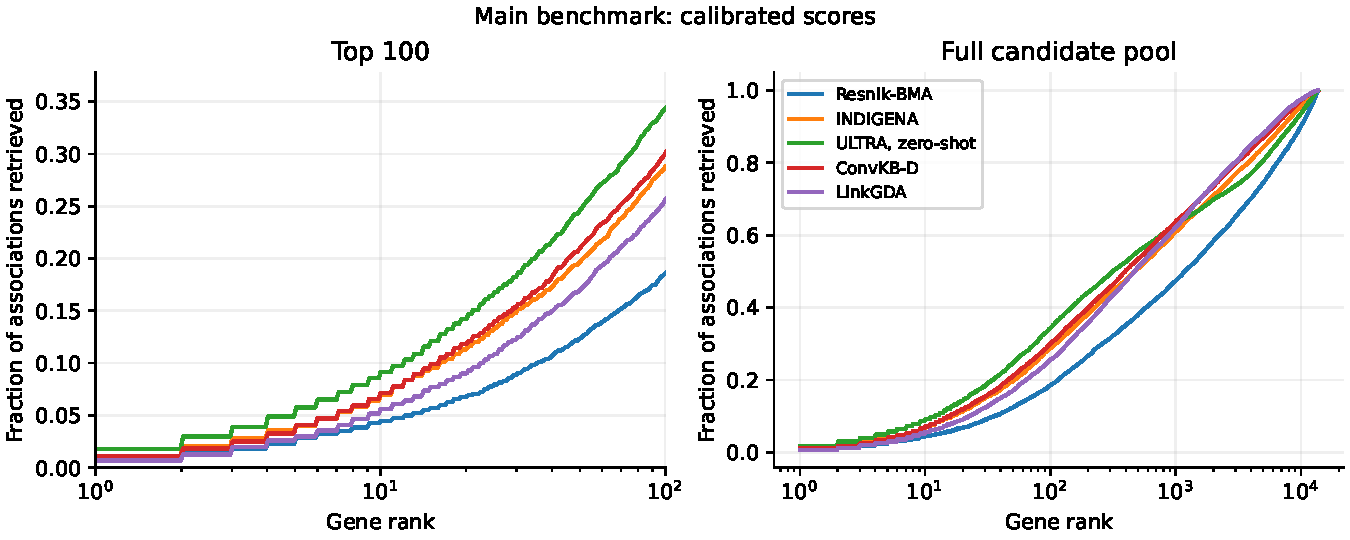
\includegraphics[width=\textwidth]{revised_rank_cdf.pdf}
\caption{Cumulative rank distributions in the main benchmark, with equal weight
per fold. All curves use disease-level calibration. The left panel expands the
top 100 positions; the right shows the full 13,625-gene pool.}
\label{fig:rank_cdf}
\end{figure*}

\subsection{Candidate status and ranking within status groups}

Association status can predict evaluation labels independently of the query
phenotypes; its contribution depends on the candidate universe.
In the annotation-defined main pool, placing training-associated genes first
gives mean rank 5{,}505; placing unseen genes first gives 8{,}121, compared
with a random-order expectation of 6{,}813. Calibrated \method{} achieves
mean rank 393 among seen candidates and 1{,}427 among unseen candidates,
compared with random-order expectations of 1{,}890 and 4{,}923. ConvKB-D
has slightly lower seen-group mean rank (387), while \method{} has the
lowest unseen-group mean rank among the compared methods. Suppl. Table~\ref{supp-tab:status}
gives all methods. These comparisons establish ranking information within
training-status groups. To test its dependence on the query, we enumerate
every other disease profile in the same fold while retaining the calibrated
scores. Expected mean rank becomes 6,772 for \method{} and 6,966 for ULTRA,
compared with the random-order reference of 6,813 (Suppl. Table~\ref{supp-tab:query_control}).

The status effect also occurs in a previously released benchmark from our
group. In
INDIGENA's public 1{,}529-mouse-gene dataset~\citep{indigena}, ranking genes
absent from training associations first gives mean rank $470.46\pm48.70$
across ten released outer folds with a reconstructed inner validation split, compared with a random-order expectation of
765. Such genes constitute 14.84\% of candidates but 53.37\% of test pairs.
This provides a second quantified example of candidate-status enrichment;
the targeted literature audit and general mean-rank identity are described
in the Supplementary Methods.

\subsection{Genes without mouse phenotype annotations}

We next ranked 425 associations from 417 diseases among 5{,}696 GO-annotated
genes without MGI phenotypes. With calibrated scores, the function-only and
function--expression \method{} variants have mean ranks 1{,}193 and 1{,}169
(Table~\ref{tab:excluded}). Relative to matched ULTRA, their mean-rank
differences are $-118$ (97.5\% disease-bootstrap interval: $-253$ to $14$)
and $-302$ ($-445$ to $-166$), respectively. The function--expression
comparison supports a lower mean rank, while the function-only interval
spans zero. Function-only \method{} recovers 12.40\% of associations in
the top ten, compared with 7.88\% for the function--expression variant.
In this cohort, adding expression improves mean rank while reducing
top-ranked retrieval. Raw ULTRA-f gives 13.65\% top-10 recovery, compared
with 11.06\% after calibration.

\begin{table*}[tb]
\centering\small
\caption{Ranking 425 associations from 417 diseases whose genes lack MGI phenotypes. Primary evaluation ranks 5,696 GO-annotated genes without MGI phenotypes; the secondary full-GO pool has 18,904 genes. Model scores use disease-level calibration; controls order uncalibrated annotation counts. MR is the mean over ten LinkGDA seeds and SD describes optimization variability; ULTRA is deterministic. Bootstrap intervals use seed-averaged pair ranks.}
\label{tab:excluded}
\begin{tabular}{lrrrr}
\toprule
Pool & Method & MR & MRR & H@10 (\%) \\
\midrule
No-MGI & LinkGDA-f & 1192.91\std{51.48} & 0.064 & 12.40 \\
No-MGI & ULTRA-f & 1311.11\std{0.00} & 0.054 & 11.06 \\
No-MGI & LinkGDA-fs & 1169.42\std{26.48} & 0.043 & 7.88 \\
No-MGI & ULTRA-fs & 1471.22\std{0.00} & 0.050 & 9.65 \\
No-MGI & GO-count control & 1571.70 & 0.005 & 0.24 \\
Full GO & LinkGDA-f & 4087.93\std{202.69} & 0.030 & 6.24 \\
Full GO & ULTRA-f & 4380.92\std{0.00} & 0.028 & 5.65 \\
Full GO & LinkGDA-fs & 3961.01\std{86.32} & 0.018 & 3.48 \\
Full GO & ULTRA-fs & 5187.51\std{0.00} & 0.019 & 4.24 \\
Full GO & GO-count control & 8573.05 & 0.000 & 0.00 \\
\bottomrule
\end{tabular}
\end{table*}


Calibration has different effects in this cohort. For the same selected
checkpoints, raw mean ranks are 1{,}083 for the function model and 856 for
the function--expression model, both lower than their calibrated values.
Calibration increases top-10 recovery from 9.53\% to 12.40\% and from
7.06\% to 7.88\%, respectively. In the full-GO sensitivity, placing genes without MGI phenotypes first gives
mean rank 2{,}848.5, lower than all calibrated model ranks in that pool.
This control quantifies the remaining annotation-status advantage in the
secondary analysis. In the primary pool every candidate lacks MGI phenotypes,
so the same rule ties all candidates at rank 2{,}848.5.

Query permutation also separates rank information from gene-level priors.
For raw \method{}-fs in the primary pool, the exact expected mean rank under
another disease query is 1,630, against 856 for the correct query. With
calibration it is 2,846, close to the random reference of 2,848.5; ULTRA-fs
gives 3,020. Part of the 302-rank comparison therefore persists under incorrect
queries. The primary contrast measures predictive ranking under this benchmark;
the permutation control identifies a residual gene-level contribution.

\subsection{Annotation sources and calibration}
\label{sec:calibration_results}

In the main benchmark, the phenotype-only model has mean rank 2{,}699.
Combining phenotype with function lowers it to 1{,}790, and combining all
three annotation types lowers it to 1{,}729. Function alone gives 2{,}410,
function with expression 2{,}058, and expression alone 3{,}748
(Suppl. Table~\ref{supp-tab:rq1_ablation}). These are sensitivity comparisons between variants with
fixed, potentially different hyperparameters. Withholding mouse phenotype
profiles retains training-derived gene--phenotype supervision and a phenotype
fallback for candidates lacking another representation.

For LinkGDA-pfs, calibration improves mean rank under either
checkpoint-selection criterion. The raw-selected checkpoint has mean rank
2{,}541 with raw scores and 1{,}721 with disease-level calibration. The
calibrated-selected checkpoint gives 2{,}538 and 1{,}729, respectively.
Fixed training-disease reference statistics give mean rank 1{,}722 for the
latter checkpoint, with 5.82\% top-10 recovery (Suppl. Table~\ref{supp-tab:calibration}). This panel
supports scoring a new disease independently of other test queries.

\section{Discussion}

PhenoQuery treats a disease phenotype set as a conjunctive query over a
relational graph. Its controlled component comparisons support removing
training disease bridges and adding typed entity--quality information for
top-ten gene retrieval. Ontology structure contributes through the learned
phenotype projections, while conjunction requires a candidate to explain
multiple query phenotypes. The evaluated procedure includes validation-based
selection between adapted and initial checkpoints. This combination provides
a practical method for ranking genes from disease profiles within the studied
candidate universe.

The evaluation also shows why a method's performance depends on the available
training information. Disease-disjoint folds contain both previously
associated genes and genes without training disease associations, and most
seen-gene test pairs share phenotypes with their training diseases. Phrank
accounts for phenotype ancestry through conditional information content and
identified optimistic estimates when simulated patient profiles are drawn from
the knowledgebase used for ranking. Its evaluation used real patient profiles
\cite{jagadeesh2019phrank}. PhenoRank
used simulated queries to address annotation and network-related biases
\cite{cornish2018phenorank}. Our analysis extends these concerns to a common
whole-gene benchmark, distinguishes training-association status from phenotype
overlap, and evaluates their interaction with graph structure and score
calibration. Gene multifunctionality, graph degree and total annotation
information also provide relevant context
\cite{gillis2011multifunctional,zietz2024degree,alghamdi2022contribution}.

Each evaluation adjustment answers a specific question. Per-gene calibration
compares a candidate's response with its responses to other phenotype queries.
Status normalization compares standardized responses across training-status
groups. Zero-overlap and unseen-gene cohorts target more demanding transfer
settings. Reference deduplication and profile weighting control the influence
of repeated phenotype descriptions, while co-causal filtering defines
competition among genes with multiple known positives. Reporting these choices
separately preserves the distinction between improved scoring and a changed
target population. Native baseline rankings remain essential because additional
normalization can reduce retrieval for an already calibrated method.

The present experiments use a disease-inductive benchmark in which candidate
genes have graph representations before test scoring. The component study is
an exploratory, single-seed comparison on folds that informed development;
its bootstrap intervals describe sampling variation conditional on the fitted
models. The historical embedding sensitivities also vary in training budget,
dimension or checkpoint selection. Matched training across those dimensions,
additional seeds and independent disease cohorts would establish broader
comparative performance. Reproduction starts from retained prepared annotation
tables and pinned ontology files because some original provider snapshots are
unavailable. Clinical validation additionally requires patient phenotypes,
variants and patient-specific candidate lists.

\section{Conclusion}

Typed entity--quality information improves PhenoQuery's top-ten gene retrieval
in a controlled component comparison. Candidate status, shared training
phenotypes and evaluation weighting substantially alter the rankings observed
on the same disease-disjoint benchmark. Combining a phenotype-query method
with explicit native-score, calibration and cohort analyses makes its predictive
contribution and generalization setting measurable.

\section*{Competing interests}
No competing interest is declared.

\section*{Author contributions statement}

F.Z.C. designed the method, conducted the experiments, wrote the software,
curated the data, and analyzed and interpreted the results. N.M.
contributed to the software, conducted experiments, and interpreted the
results. R.H. conceived of and supervised the work, contributed to the
methodology, provided resources, and acquired funding. All authors wrote
and critically revised the manuscript.

\section*{Funding}
This work has been supported by funding from King Abdullah University
of Science and Technology (KAUST) Office of Sponsored Research (OSR)
under Award No. URF/1/4675-01-01, URF/1/4697-01-01, URF/1/5041-01-01,
REI/1/5235-01-01, and REI/1/5334-01-01. This work was supported by
funding from KAUST -- KAUST Center of Excellence for Smart Health
(KCSH), under award number 5932, and by funding from KAUST -- Center of
Excellence for Generative AI, under award number 5940.

\section*{Data availability}
The data come from public sources as described in Section~\ref{sec:datasets}.
Source code is maintained at
\url{https://github.com/bio-ontology-research-group/link-gda}.
The frozen prepared-input release is available at
\url{https://github.com/bio-ontology-research-group/link-gda/releases/tag/inputs-20261028-v1}.
The reproduction repair is maintained on branch
\texttt{fix/phenoquery-reproducibility}. Experiment manifests identify the
prepared annotation snapshots, ontology inputs, split identities and saved
score arrays used in each analysis.


%UNCOMMENT THE BELOW TWO LINES IN CASE YOU NEED NUMBERED FORMAT.
%\bibliographystyle{oup-plain}
%\bibliography{reference}

%UNCOMMENT THE BELOW TWO LINES IN CASE YOU NEED AUTHOR YEAR FORMAT.
\bibliographystyle{oup-abbrvnat-short}
\bibliography{reference}

% REVIEW (applied): the OUP sample author-biography boilerplate was removed
% (commented out). Bioinformatics research papers do not carry author
% biographies; leaving the placeholder text would appear in the PDF.
%% sample for biography with author's image
%\begin{biography}{{\color{black!20}\rule{77pt}{57pt}}}{\author{Author Name.} This is sample author biography text. The values provided in the optional argument are meant for sample purposes. There is no need to include the width and height of an image in the optional argument for live articles. This is sample author biography text this is sample author biography text this is sample author biography text this is sample author biography text this is sample author biography text this is sample author biography text this is sample author biography text this is sample author biography text.}
%\end{biography}

%% sample for biography without author's image
%\begin{biography}{}{\author{Author Name.} This is sample author biography text this is sample author biography text this is sample author biography text this is sample author biography text this is sample author biography text this is sample author biography text this is sample author biography text this is sample author biography text.}
%\end{biography}

%%%%%%%%%%%%%%


\end{document}
